\chapter{Density functional theory} \label{Density functional theory}

\section{Introduction}
Amongst the most used methods in computational chemistry nowadays, especially for research on industrially relevant compounds, are the ones based on density functional theory (DFT), that is the methods in which one computes the electron density $\rho$, instead of the wave function $|\Psi\rangle$, of the system. The motivation for this is that the wave function of an $N$ electrons system depends on $3N$ spatial coordinates and $N$ spin coordinate, while the electron density is the square of the wave function, integrated over $N-1$ electron coordinates, thus while the complexity of the wave function increases exponentially with the number of electrons, the electron density has the same number of variables, independent of the system size.
\begin{equation}
    \rho({\bf {r}}) = N \sum_{s_1,...,s_N} \int d{\bf r}_2...d{\bf r}_N |\Psi({\bf r},s_1,{\bf r}_2,s_2,...,{\bf r}_N,s_N)|^2
\end{equation}
The electron density can be linked to all the properties of the Hamiltonian and therefore of the atomic system. First of all, by integrating it over all space we can get the total number of electrons $N$,
\begin{equation}
    N = \int \rho({\bf r})d{\bf r}.
\end{equation}
Secondly, it is possible to get information about the nuclei via the formula
\begin{equation}
    \frac{\partial \bar{\rho} (r_A)}{\partial r_A}\bigg|_{{\bf r}_A=0} = -2Z_A \rho({\bf r}_A),
\end{equation}
where $Z$ is the atomic number, $r_A$ is the radial distance and $\bar{\rho}$ is the spherically averaged density. \\
This is not a simple formalism for finding the energy, but it shows that given a known density, one could form the Hamiltonian operator, solve the TISE and determine the wave function along with the energy eigenvalues.

\section{First approach}
The simplest approach to this calculation is to consider the system to be classical and provide the total energy as a sum of kinetic and potential energy. \\
The potential energy components are easily determined. The attraction between the density and the nuclei is
\begin{equation}
    V_{ne} [\rho({\bf r})] = \sum_I^{nuclei} \int \frac{Z_I}{|{\bf r} - {\bf r}_I|}\rho({\bf r})d{\bf r},
\end{equation}
and the self-repulsion of a classical charge distribution is
\begin{equation}
    V_{ee} [\rho({\bf r})] = \frac{1}{2} \iint\frac{\rho({\bf r}_i) \rho({\bf r}_j)}{|{\bf r}_i - {\bf r}_j|} d{\bf r}_i d{\bf r}_j. \label{V_ee}
\end{equation}
For the kinetic energy we can use the result of Thomas and Fermi from 1927 for the jellium model, i.e. a system composed of electrons moving in an infinite volume characterized by a uniformly distributed positive charge, also called uniform electron gas,
\begin{equation}
    T_{jellium} [\rho({\bf r})] = \frac{3}{10}(3\pi^2)^{2/3} \int \rho^{5/3}({\bf r}) d{\bf r}.
\end{equation}
These functions depends on density $\rho$ which in turn depends on position $\bf r$, for this reason $T$ and $V$ are called density functionals. \\
The Thomas-Fermi equations, together with an assumed variational principle, represented the first effort to define a density functional theory, the energy is computed with no reference to a wave function. \\
\\
However this formulation is highly inaccurate, due to the large approximation on the interelectronic repulsion, eq. (\ref{V_ee}), which does not take into account the effects associated with correlation and exchange. \\
A hole function can be introduced to correct for the energetic errors introduced by assuming classical behaviour, this acts like a negative density. \\
In the following years Slater suggested to consider a functional for the exchange term by approximating the exchange hole as a sphere of constant potential with a radius depending on the magnitude of the density at that position
\begin{equation}
    E_{x} [\rho({\bf r})] = -\frac{9 \alpha}{8} \left( \frac{3}{\pi} \right)^{1/3} \int \rho^{4/3}({\bf r}) d{\bf r},
\end{equation}
this is called the Slater exchange. Within Slater's derivation the value of $\alpha$ is 1. \\
Later on, Bloch and Dirac derived a similar expression with $\alpha = \frac{2}{3}$. The combination of these expressions defines the Thomas-Fermi-Dirac model, although it too remains sufficiently inaccurate for modern use. \\
Early DFT models found widespread use in the solid state physics community, however had little impact on chemistry due to large errors in molecular calculation and the failure to provide a rigorous foundation.

\section{Analysis}

\subsection{Hohenberg-Kohn theorems}
In 1964 Hohenberg and Kohn proved two theorems that estabilished the legitimacy for DFT as a computational chemistry method.

\begin{enumerate}
    \item \textit{The ground state electron density $\rho_0$ completely determines the external potential.}
\end{enumerate}
This is also called 'the existence theorem', because it proves the existence of a density function that satisfies the properties we want. \\
The external potential represents the attraction between the electron density and the nuclei. The proof proceeds via $reductio \ ad \ absurdum$ and takes advantage of the variational principle for the ground state energy from quantum mechanics \cite{Cramer2004Sep}. \\
If the electron density determines the external potential then it determines the Hamiltonian and therefore the wave function of the system.

\begin{enumerate}
    \setcounter{enumi}{1}
    \item \textit{For any positive density $\rho$, such that $\int \rho({\bf r})d{\bf r} = N$,}
    \begin{equation}
        \langle\Psi(\rho)|H(\rho)|\Psi(\rho)\rangle = E(\rho) \geq E_0
    \end{equation}
\end{enumerate}
This is also called the 'variational theorem', because it provides a variational principle for the electron density function. \\
Just as the HF-based methods, generally called molecular orbital (MO) theory, we need a means to optimize the quantity we aim to find. This theorem shows that the density obeys a variational principle. So we can keep choosing different densities and those that provide lower energies are closer to the correct one, but we have no means to improve the candidate density that we choose. \\
\\
These two theorems make a solid foundation for DFT, since there is a formal way that we can get the energy values of the system, but we still can not avoid solving the TISE, which is the motivation for which we study DFT. So we need further refinement to the method in order to use it. \\
Note also that the Hamiltonian determines not just the ground state wave function, but all the excited state wave functions as well, so there is an enormous amount of information coded in the density.

\subsection{Kohn-Sham self-consistent field method}
In 1965 Kohn and Sham described a method to find energy values using DFT. \\
We know that the Hamiltonian for a non-interacting system of electrons: can be expressed as a sum of one-electron operators, has eigenfunctions that are Slater determinants of the individual one-electron eigenfunctions and has eigenvalues that are simply the sum of the one-electron eigenvalues. So we take a fictitious system of non-interacting electrons that have, for their overall ground state density, the same density as some real system of interest where electrons do interact. We know we can do that because the density determines the position and the atomic numbers of the nuclei and these quantities are necessarily identical. \\
The energy functional can be written as
\begin{equation}
    E[\rho({\bf r})] = T_{ni}[\rho({\bf r})] + V_{ne}[\rho({\bf r})] + V_{ee}[\rho({\bf r})] + \Delta T[\rho({\bf r})] + \Delta V_{ee}[\rho({\bf r})], \label{KS}
\end{equation}
where $ni$ stands for $non$-$interacting$ and $\Delta T$ and $\Delta V_{ee}$ are the corrections to the kinetic energy and to the electron-electron repulsion energy, due to non-classical terms of interactions between particles that arises from quantum mechanical treatment. Those are the terms we have to add to the non-interacting system to regain the real system. \\
This is a useful formulation becuase we already know the form of kinetic and potential energy from the classical scheme. However, the cost of this facilitation is that we have to reintroduce orbitals function to give an exact definition of these functionals, in contrast with first approaches to DFT where kinetic and potential energy were completely defined by density but the model used to define them was approximated. This means that the complexity of the method increases from $3$ to $3N$ spatial variables. \\
We can rewrite eq. (\ref{KS}) as
\begin{equation}
\begin{split}
    E[\rho({\bf r})] = \sum_i^N \left( \langle\chi_i| - \frac{1}{2} \nabla_i^2 |\chi_i\rangle - \langle\chi_i|\sum_I^{nuclei} \frac{Z_I}{r_{iI}} |\chi_i\rangle \right) \\
    + \sum_i^N \left( \langle\chi_i| \frac{1}{2} \int \frac{\rho({\bf r}')}{|{\bf r}_i - {\bf r}'|} d{\bf r}' |\chi_i\rangle \right) + E_{xc}[\rho({\bf r})],
\end{split}
\end{equation}
where the density for the exact eigenfunction for the non-interacting system, i.e. a Slater-determinantal wave function, is
\begin{equation}
    \rho = \sum_i^N \langle\chi_i|\chi_i\rangle.
\end{equation}
The corrections we have introduced have been grouped under $E_{xc}[\rho({\bf r})]$, which is called the 'exchange-correlation energy' or the 'exchange-correlation functional'. This term includes not only the effects of quantum mechanical exchange and correlation, but also the correction for the classical self-interaction energy and for the difference in kinetic energy between the fictitious non-interacting system and the real one. \\
As we have done before with the HF method we can find the orbitals $|\chi_i\rangle$ that minimze the energy $E$. To do this we can write the pseudoeigenvalue equations as
\begin{equation}
    h^{KS}_i |\chi_i\rangle = \epsilon_i |\chi_i\rangle,
\end{equation}
where
\begin{equation}
    h^{KS}_i = -\frac12\nabla^2_i -\sum_I^{nuclei}\frac{Z_I}{r_{iI}} + \int \frac{\rho({\bf r}')}{|{\bf r}_i - {\bf r}'|} d{\bf r}' + V_{xc}
\end{equation}
is the Kohn-Sham (KS) one-electron operator, defined in an analogous way to the Fock operator, and
\begin{equation}
    V_{xc} = \frac{\delta E_{xc}}{\delta \rho}
\end{equation}
is a functional derivative. \\
Since the functional $E$ we are minimizing is exact (we know that because we have considered a simple system) the orbitals $|\chi_i\rangle$ must provide the exact density of the real system. Furthermore, these orbitals are the correct ones to form the Slater-determinantal eigenfunction for the separable non-interacting Hamiltonian defined as the sum of the KS operators,
\begin{equation}
    \sum_i^N h^{KS}_i |\chi_1 \chi_2 ... \chi_N\rangle = \sum_i^N \epsilon_i |\chi_1 \chi_2 ... \chi_N\rangle.
\end{equation}
It is therefore justified the use of the fictitious non-interacting system we have introduced before \cite{Cramer2004Sep}. \\
To obtain the KS orbitals we follow the same path developed for MO theory, we express them within a basis set of functions $\{ |\phi_{\nu}\rangle \}$ and we determine the individual orbital coefficients by solution of a secular equation analogous to the one for HF theory except that the elements $F_{\mu \nu}$ are replaced by $K_{\mu \nu}$ defined as
\begin{equation}
    K_{\mu \nu} = \langle\phi_{\mu}| \left( -\frac12\nabla^2_i -\sum_I^{nuclei}\frac{Z_I}{r_{iI}} + \int \frac{\rho({\bf r}')}{|{\bf r}_i - {\bf r}'|} d{\bf r}' + V_{xc} \right) |\phi_{\nu}\rangle. \label{K mu nu}
\end{equation}
Now that we have defined the target of the method we have to define the procedure to obtain it. \\
We take advantage of the second HK theorem, i.e. the variational principle, and define the procedure as follow:
\begin{enumerate}
    \item \textbf{Choose a basis set,} sometimes orbitals and density use different basis sets;
    \item \textbf{Choose a molecular geometry;}
    \item \textbf{Compute overlap and one-electron integrals;}
    \item \textbf{Guess initial density,} this can be constructed as a matrix;
    \item \textbf{Construct and solve KS secular equation;}
    \item \textbf{New orbitals are determined from the solution, from these construct the new density;}
    \item \textbf{Compare the two densities.} \\
    If they are sufficiently similar compute the energy by plugging the final density in eq. ($\ref{KS}$), this is in contrast with HF theory where the energy is evaluated as the expectation value of the Hamiltonian operator acting on the HF Slater determinant, otherwise repeat from 5;
    \item \textbf{Optional: optimize molecular geometry}, i.e. determine if the structure corresponds to a stationary point.
\end{enumerate}
Due to the repetition and the similar structure to HF method, this procedure is also called KS self-consistent field (SCF) method. \\
The scheme is depicted in Figure \ref{KS method}. \\
\begin{figure}[ht]
  \centering
  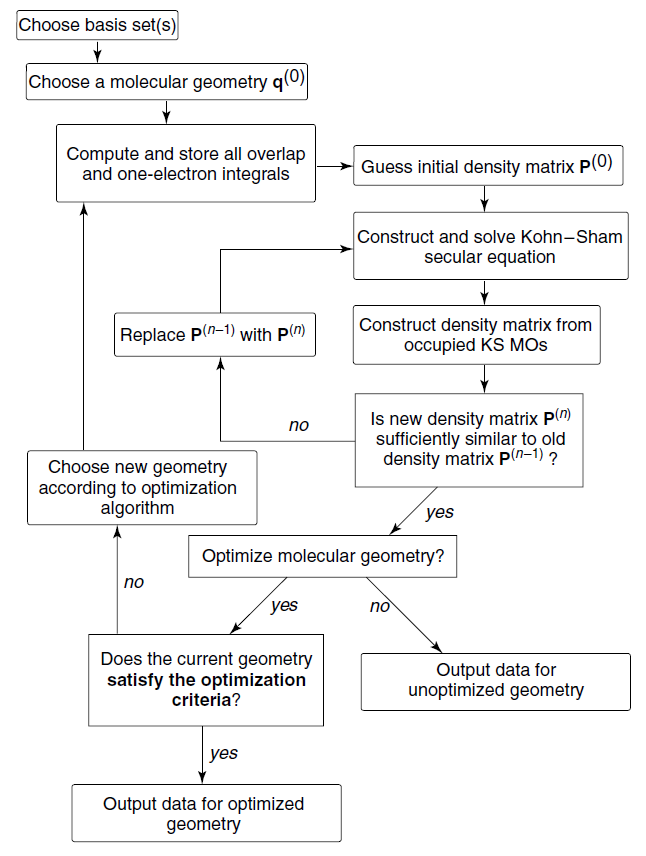
\includegraphics[width=0.75\textwidth]{figures/KS method.png}
  \caption{Flowchart for the KS SCF method \cite{Cramer2004Sep}.} \label{KS method}
\end{figure} \\
There is a key difference between HF theory and DFT. HF is a deliberately approximate theory, whose development was in part motivated by an ability to solve the relevant equations exactly. DFT, instead, contains no approximation, all we need to know is $E_{xc}$ as a function of $\rho$. However while Hohenberg and Kohn proved that a functional of the density must exist, their proofs provide no guidance whatsoever as to its form. As a result, considerable research effort has gone into finding functions of the density that may be expected to reasonably approximate $E_{xc}$. Therefore, DFT is an exact theory, but the relevant equations must be solved approximately because a key operator has unknown form.

\subsection{Exchange-correlation functionals}
From the first version of DFT hundreds of different exchange-correlation functionals have been introduced. Here we will show some of the most important ones. \\
First of all, the functional is expressed as an interaction between the electron density and an energy density, that is dependent on the electron density
\begin{equation}
    E_{xc}[\rho({\bf r})] = \int \rho({\bf r}) \epsilon_{xc}[\rho({\bf r})] d{\bf r},
\end{equation}
and the energy density $\epsilon_{xc}$ is treated as a sum of individual exchange, $\epsilon_x$, and correlation, $\epsilon_c$, contributions. As an example, the Slater exchange energy density is
\begin{equation}
    \epsilon_{x} [\rho({\bf r})] = -\frac{9 \alpha}{8} \left( \frac{3}{\pi} \right)^{1/3} \rho^{1/3}({\bf r}). \label{Slater}
\end{equation}
For simplicity we will not consider spin polarization, although it is possible to formulate the functional to account for it. \\
An important consideration is that, although we do not know the form of the exact functional, we know a number of properties that it should have: \cite{Jensen2011Dec}
\begin{enumerate}
    \item The energy functional should be self-interaction-free, i.e. the exchange energy for a one-electron system, such as the hydrogen atom, should exactly cancel the Coulomb energy, and the correlation energy should be zero;
    \item When the density becomes constant, the uniform electron gas result should be recovered;
    \item The coordinate scaling of the exchange energy should be linear, i.e. multiplying the electron coordinates with a constant factor should result in a similar linear scaling of the exchange energy;
    \item No direct scaling law applies for the correlation energy, but scaling the electron coordinates by a factor larger than 1 should increase the magnitude of the correlation and viceversa. In the low density limit, the scaling becomes linear, as for the exchange energy;
    \item As the scaling parameter goes to infinity, the correlation energy for a finite system approaches a negative constant;
    \item The Lieb–Oxford condition places an upper bound for the exchange–correlation energy relative to the Local density approximation (LDA) exchange energy
    \begin{equation}
        E_x[\rho({\bf r})] \geq E_{xc}[\rho({\bf r})] \geq 2.273 E_x^{LDA}[\rho({\bf r})];
    \end{equation}
    \item The exchange potential should show an asymptotic $-r^{-1}$ behaviour as $r \xrightarrow[]{} \infty$. Furthermore, the exchange–correlation potential is discontinous as a function of the number of electrons, by an amount corresponding to the difference between the ionization potential and electron affinity;
    \item The correlation potential should show an asymptotic $-\frac{1}{2} \alpha r^{-4}$ behaviour, with $\alpha$ being the polarizability of the $N_{elec} - 1$ system.
\end{enumerate}
The first type of functionals we study is the one derived from the uniform electron gas, where the density has the same value at every position, this type is also called local density approximation (LDA), to express that the value of $\epsilon_{xc}$ at some position ${\bf r}$ could be computed exclusively from the value of $\rho$ at that position, i.e the local value of $\rho$. \\
As discussed before the exchange energy for the uniform electron gas can be computed exactly and is given by eq. (\ref{Slater}), where $\alpha$ can take different values based on the model considered. \\
Systems including spin polarization, e.g. open-shell systems, must use spin-polarized formalism, and its greater generality is sometimes distinguished with the expression local spin density approximation (LSDA). \\
As for the correlation energy density no analytical derivation of this functional has been proven possible and it is sometimes computed via quantum Monte Carlo techniques. \\
\\
One obvious way to improve the correlation functional is to make it depend not only on the local value of the density, but on the extent to which the density is locally changing, i.e. the gradient of the density. The more common term in modern nomenclature for functionals that depend on both the density and the gradient of the density is ‘gradient corrected’. Including a gradient correction defines the ‘generalized gradient approximation’ (GGA). \\
Most gradient corrected functionals are constructed with the correction being a term added to the LDA functional, i.e.
\begin{equation}
    \epsilon_{x/c}^{GGA} [\rho({\bf r})] = \epsilon_{x/c}^{LDA} [\rho({\bf r})] + \Delta \epsilon_{x/c} \left[ \frac{|\nabla \rho({\bf r})|}{\rho^{4/3}({\bf r})} \right]. \label{GGA}
\end{equation}
The first widely popular GGA exchange functional was developed by Becke and it is usually abbreviated simply B. It further incorporates a single empirical parameter the value of which was optimized by fitting to the exactly known exchange energies of the six noble gas atoms He through Rn. \\
Other exchange functionals similar to the Becke example, in one way or another, have appeared, including CAM, FT97, O, PW, mPW, and X, where X is a particular combination of B and PW found to give improved performance over either. \\
Alternative GGA exchange functionals have been developed based on rational function expansions of the reduced gradient. These functionals, which contain no empirically optimized parameters, include B86, LG, P, PBE, and mPBE. \\
With respect to correlation functionals, corrections to the correlation energy density following eq. ($\ref{GGA}$) include B88, P86, and PW91. \\
Another popular GGA correlation functional, LYP, does not correct the LDA expression but instead computes the correlation energy in toto. It contains four empirical parameters fit to the helium atom. Of all of the correlation functionals discussed, it is the only one that provides an exact cancellation of the self-interaction error in one-electron systems. \\
Typically in the literature, a complete specification of the exchange and correlation functionals is accomplished by concatenating the two acronyms in that order. Thus, for instance, a BLYP calculation combines Becke’s GGA exchange with the GGA correlation functional of Lee, Yang, and Parr. \\
The next step in functional improvement might be to take account of the second derivative of the density, i.e., the Laplacian. Such functionals are termed meta-GGA (MGGA) functionals as they go beyond simply the gradient correction. However, numerically stable calculations of the Laplacian of the density pose something of a technical challenge, and the somewhat improved performance of MGGA functionals over GGA analogs is balanced by this slight drawback. \\
An alternative MGGA formalism that is more numerically stable is to include in the exchange-correlation potential a dependence on the kinetic-energy density $\tau$, defined as
\begin{equation}
    \tau ({\bf r}) = \sum_i^{occupied} \frac{1}{2} |\nabla \chi_i ({\bf r})|^2,
\end{equation}
where the $\chi_i$ are the self-consistently determined KS orbitals. \\
\\
Antoher imporant type of functional is defined by the adiabatic connection method (ACM). \\
Let's imagine we have a parameter $\lambda$ we can tune to smoothly convert the non-interacting KS reference system to the real, interacting system. Using the Hellmann–Feynman theorem, one can show that the exchange-correlation energy can then be computed as
\begin{equation}
    E_{xc} = \int_0^1 \langle\Psi(\lambda)|V_{xc}(\lambda)|\Psi(\lambda)\rangle d\lambda.
\end{equation}
To evaluate this integral, it is helpful to adopt a geometric picture, as shown in Figure \ref{Adiabatic connection method}.
\begin{figure}[ht]
  \centering
  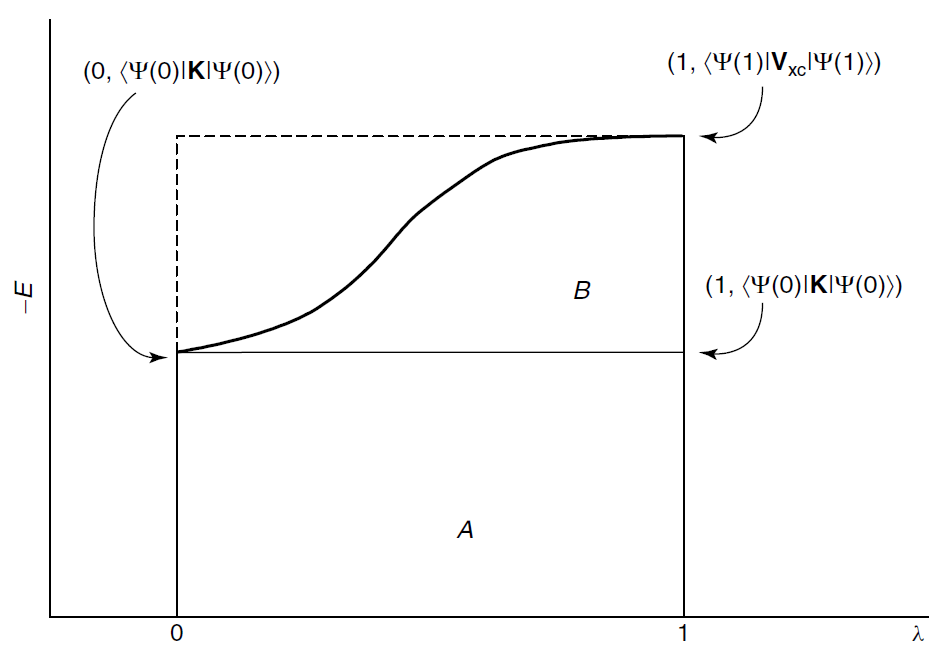
\includegraphics[width=0.75\textwidth]{figures/Adiabatic connection method.png}
  \caption{Geometrical scheme for the exchange-correlation energy \cite{Cramer2004Sep}.} \label{Adiabatic connection method}
\end{figure} \\
We seek the area under the curve defined by the expectation value of $V_{xc}$. While we know very little about $V$ and $\ket{\Psi}$ as functions of $\lambda$ in general, we can evaluate the left endpoint of the curve. In the non-interacting limit, the only component of $V$ is exchange (deriving from antisymmetry of the wave function). Moreover, the Slater determinant of KS orbitals is the exact wave function for the non-interacting Hamiltonian operator. Thus, the expectation value is the exact exchange for the non-interacting system, which can be computed just as it is in HF calculations except that the KS orbitals are used. The total area under the expectation value curve thus contains the rectangle having the curve’s left endpoint as its upper left corner, which has area $E_x^{HF}$. \\
The remaining area is some fraction $z$ of the area corresponding to the rectangle sitting immediately on top of the first; the second rectangle has area $\langle\Psi(1)|V_{xc}(1)|\Psi(1)\rangle - E_x^{HF}$. Unfortunately, not only do we not know $z$, we also do not know the expectation value of the fully interacting exchange-correlation potential applied to the fully interacting wave function. However, we may regard $z$ as an empirical constant to be optimized. In that case, we may as well approximate the unknown right endpoint, and a convenient approximation is the $E_{xc}$ computed directly by some choice of DFT functional. \\
We see then that the total area under the expectation value curve can be written as
\begin{equation}
    E_{xc} = E_x^{HF} + z(E_{xc}^{DFT} - E_x^{HF}) = (1-a)E_{xc}^{DFT} + aE_x^{HF},
\end{equation}
where $a = 1-z$. \\
The transition from one system to another one makes the ACM similar to the KS SCF scheme. In the latter case, one does not know the exact kinetic energy as a function of the density, so one employs a scheme where a large portion of it is computed exactly (as the expectation value of the kinetic energy operator over the KS determinant) and worries later about the small remainder. So too, the ACM approach computes a large fraction of the total exchange-correlation energy, and then worries later about the difference between the total and the exact (HF) exchange. \\
We may also think whether inclusion of additional empirical parameters results in sufficient improvement to make such inclusion worthwhile. Becke was the first to do this, developing the 3-parameter functional expression
\begin{equation}
    E_{xc}^{B3PW91} = (1-a)E_x^{LSDA} + aE_x^{HF} + b\Delta E_x^B + E_c^{LSDA} + c\Delta E_c^{PW91},
\end{equation}
where $a$, $b$ and $c$ were optimized to 0.20, 0.72 and 0.81. \\
A similar model is the B3LYP model, defined as
\begin{equation}
    E_{xc}^{B3LYP} = (1-a)E_x^{LSDA} + aE_x^{HF} + b\Delta E_x^B + (1-c)E_c^{LSDA} + c\Delta E_c^{LYP},
\end{equation}
where $a$, $b$ and $c$ have the same values as in B3PW91. Of all modern functionals, B3LYP has proven the most popular to date \cite{Burke2012Apr}. \\
Because they incorporate HF and DFT exchange, ACM methods are also called hybrid
methods. \\
\\
Another possible type of functionals is the double-hybrid, i.e. where we combine LDA-type functionals with HF energy and post-HF energy functionals. \\
\\
Finally, one of the latest type of functionals is the Minnesota Functionals (Myz). This is a group of highly parameterized approximate exchange-correlation energy functionals. These functionals are based on the meta-GGA approximation, i.e. they include terms that depend on the kinetic energy density $\tau$, and are all based on complicated functional forms parametrized on high-quality benchmark databases, some examples are: M05, M05-2X, M06-L, M06-2X, M08-HX, M11, M12-L, M15.

\section{Computational requirements}
Let's now evaluate the scaling, the advantages and the disadvantages of the DFT method. \\
In the KS SCF method, if we write the density with an auxiliary basis set as
\begin{equation}
    \rho({\bf r}) = \sum_{i=1}^{m'} c_i \Omega_i ({\bf r}),
\end{equation}
we can find that the number of Coulomb integrals requiring evaluation in order to compute all the KS matrix elements in eq. (\ref{K mu nu}) is formally $O(m^2 m')$, where $m$ is the number of KS atomic orbital basis functions, instead of $O(m^4)$, as for HF theory. As a result, the formal bottleneck in solving the KS SCF equations is matrix diagonalization, which scales as $O(m^3)$, and one frequently sees in the literature reference to this total scaling behavior associated with DFT. \\
Compared to HF theory, DFT includes electron correlation and does so in a fashion that scales more favorably with respect to system size. However, many electronic structure programs do not employ auxiliary basis sets to represent the density, choosing instead to compute it in the HF-like way as a product of KS-orbital basis functions (the motivation for this choice was primarily historical: existing HF codes could be easily modified to carry out DFT calculations with this choice), in which case formal $O(m^4)$ scaling is not reduced. \\
Therefore the scaling is, in principle, no worse than $O(m^3)$, but if we use a hybrid method, e.g. with the B3LYP functional, we pass through the calculation of the HF energy thus the scaling of the method rise to $O(m^4)$, as we have seen before. \\
\\
The local density approximation is very simple and remarkably reliable for the structure, elastic moduli and relative phase stability of many materials, but is less accurate for binding energies and details of the energy surface away from equilibrium geometries, e.g. transition states. The GGA family of functionals improves binding energies to average errors of 20 kcal/mol and relative errors of 3-7$\%$ while meta-GGA and hybrid-exchange functionals reduce these errors to 3-5 kcal/mol and 2-3$\%$. This is close to the accuracy required for predictive simulations of thermochemical properties, i.e chemical accuracy (1 kcal/mol). The GGA, meta-GGA and hybrid functionals retain, and somewhat improve on, the LDA’s excellent description of bonds lengths with typical errors in the region of 1-2 milli-Angstrom. Using these functionals elastic moduli are reproduced to within 10$\%$ and vibrational frequencies to $\sim$ 40cm$^{-1}$. There is a distinct tendency for functionals that are highly parameterised and fitted to the properties of molecular systems to perform somewhat better than lightly parameterised functions for molecules, but to perform relatively poorly in simulations on periodic materials \cite{BibEntry2006Aug}. \\
\\
The main limitation of DFT method is that it fundamentally depends of the functional one uses. Every year new functionals are defined and the accuracy the method can reach depends on the functional choosen and even for the specific system one wants to simulate. This means that if one use the simplest functionals there is no guarantee to improve the result by using a more complicated functional. The DFT method has no systematic improvability. \\
The other limitation we already underlined is that it gives an exact solution, but the equations must be solved approximately because the form of the functional is approximated. This means that the solution will not be exact, thus we can only consider a minimum accuracy target to reach. \\
Moreover, as there are more well-characterized operators then there are generic property functionals of the density, wave functions clearly have broader utility. As a simple example, consider the total energy of interelectronic repulsion. Even if we had the exact density for some system, we do not know the exact exchange-correlation energy functional, and thus we cannot compute the exact interelectronic repulsion. However, with the exact wave function it is a simple matter of evaluating the expectation value for the interelectronic repulsion operator to determine this energy, 
\begin{equation}
    E_{ee} = \langle\Psi| \frac12 \sum_{i \neq j} \frac{1}{r_{ij}} |\Psi\rangle
\end{equation}
Another key example is in the area of dynamics, where transition probabilities depend on matrix elements between different wave functions. Because densities do not have phases as wave functions do, multistate resonance effects, interference effects, etc., are not readily evaluated within a DFT formalism. In practice, however, one can use KS orbitals, whose shapes tend to be remarkably similar to canonical HF molecular orbitals, and they can be quite useful in qualitative analysis of chemical properties, but nevertheless they represent an approximation of the solution to the TISE. \\
Lastly, dependently on the functional used one can have problems in finding specific properties of the system, e.g. older popular functionals have deficiencies in estimating barrier heights, transition metal bond energies and noncovalent interactions, as shown in Figure \ref{Comparison DFT}. \\
\begin{figure}[ht]
  \centering
  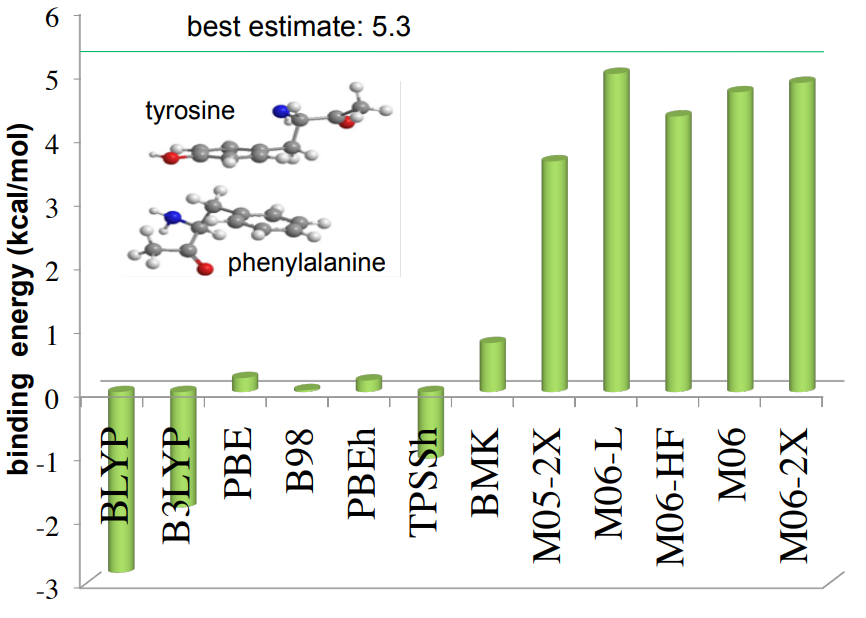
\includegraphics[width=0.75\textwidth]{figures/Comparison DFT.png}
  \caption{Comparison of the results from different functionals.} \label{Comparison DFT}
\end{figure} \\
DFT is one of the most used methods in computational chemistry, it can reach a good level of accuracy while dealing with low scaling with respect to system size. This is why it is the method we take as a standard to compare the algorithms which runs on quantum computers. \\
\begin{figure}[ht]
  \centering
  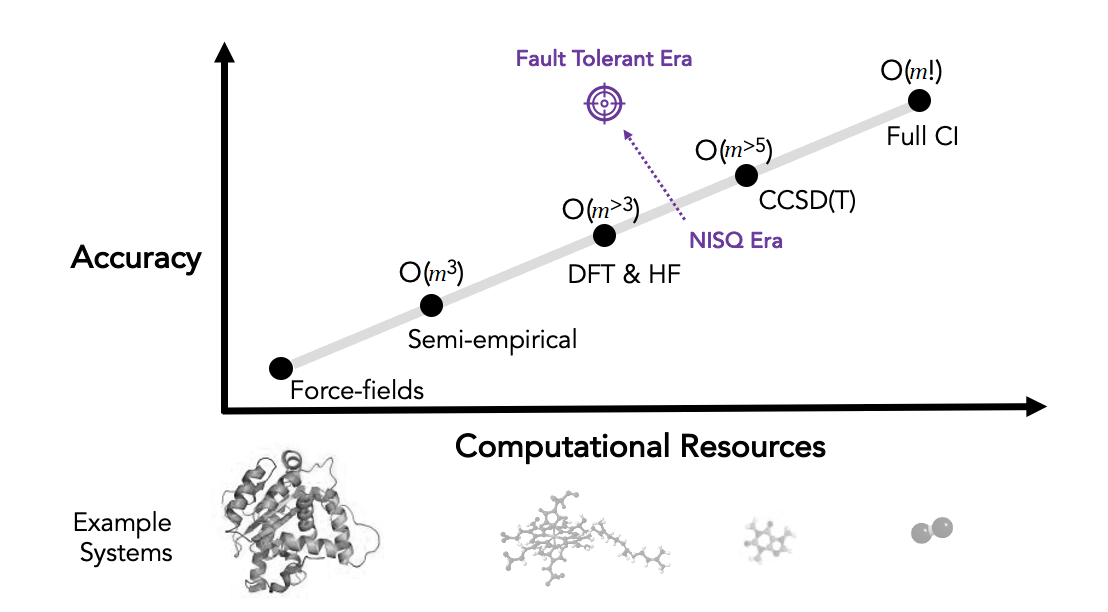
\includegraphics[width=\textwidth]{figures/Limitations of classical quantum simulations - Copia.png}
  \caption{Accuracy vs Computational resources of the main algorithms.} \label{Accuracy vs Computational resources}
\end{figure}
\\
In Figure \ref{Accuracy vs Computational resources} the main algorithms used for quantum simulation on a classical computer are depicted. The algorithms previously described are the ones that achieve a high level of accuracy up to the highest accuracy for the FCI method, but there are also cheaper methods which we did not covered. \\
The aim of quantum simulation on quantum computers is to find a method with either higher accuracy or lower computational resources compared to the already existing ones, this is represented by the purple arrow.